{\let\clearpage\relax \chapter{Control of 3 Degree of Freedom}}
	This setup was only made possible thanks to Kalman filtering since the third encoder was not working. Thus, every experiment which follows in this chapter makes use of a Kalman observer in order to estimate the position of the third cart.
\section{LQG Control Design}

The structure of this control scheme is the same as the 1 degree of freedom scenario and it is discussed in the previous chapter. In this section we only show the tuning and final results.\\

Obviously the state matrix includes also the other two carts and we must take that into account when tuning the weights on $Q$, whilst the weight on the control input $R$ is again scalar. The final tuning was output of a trial and error approach which led to the matrices
\begin{equation}
\renewcommand{\arraystretch}{1}
Q = 
\begin{bmatrix}
0 & 0 & 0 & 0 & 0 & 0 & 0\\
0 & 0 & 0 & 0 & 0 & 0 & 0\\
0 & 0 & 0.1 & 0 & 0 & 0 & 0\\
0 & 0 & 0 & 0.1 & 0 & 0 & 0\\
0 & 0 & 0 & 0 & 0 & 0 & 0\\
0 & 0 & 0 & 0 & 0 & 0 & 0\\
0 & 0 & 0 & 0 & 0 & 0 & 0\\
\end{bmatrix}
\qquad
R=1
\end{equation}
which weights the positions of the second and third carts, being the state vector defined as $x = \left[ i,\, x_1,\, x_2,\, x_3,\, \dot{x}_1,\, \dot{x}_2,\, \dot{x}_3 \right] $. We needed to weight also $x_2$ because the cart was presenting some oscillations in the transient which were due to the too strong control action.\\

Since we are not including any integral action, we need to consider a compensator on the reference which can guarantee zero error at steady state. This gain is computed as the inverse of the dc gain of the controlled plant.

\begin{figure}[h]
\centering
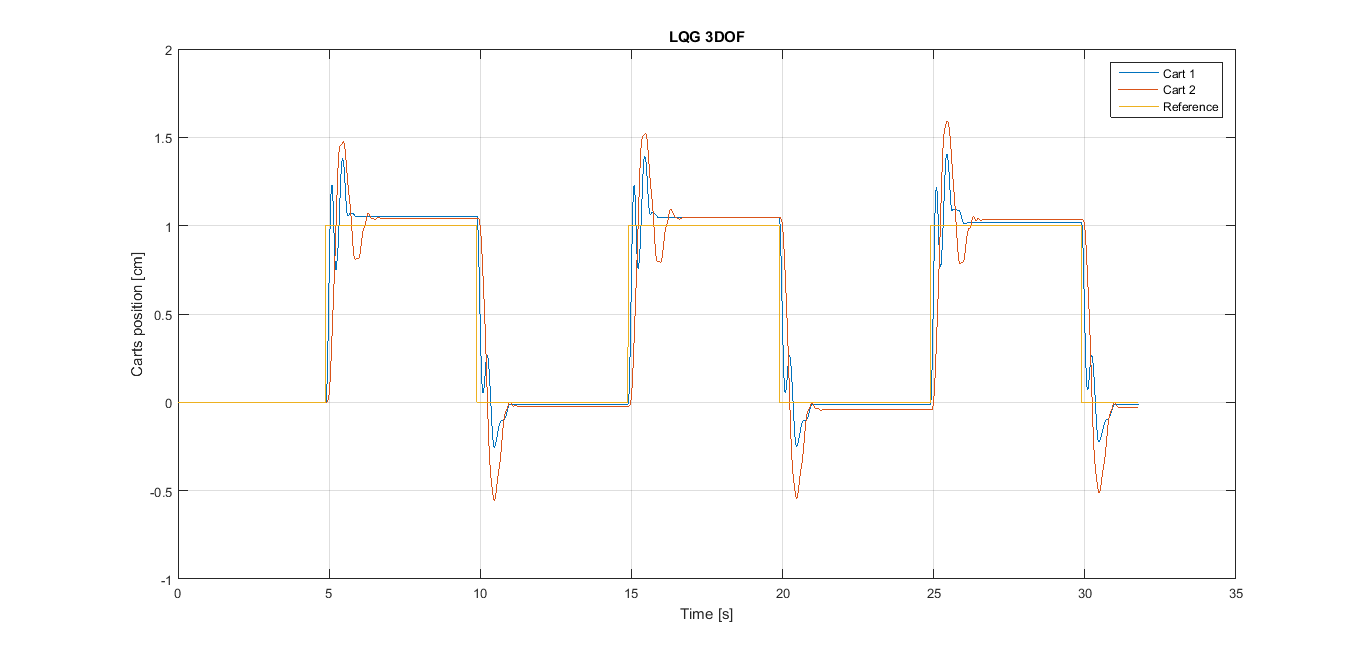
\includegraphics[width=0.5\linewidth]{img/lqg.png}
\caption{Openloop frequency response from the motor input to the position of the second cart in the case of low and medium springs employed.}
\label{fig:lqg3dof}
\end{figure}

\newpage

\section{$H_\infty$ Control Design}

The control scheme is no different from the one presented in the previous chapter; we then refer to those wrt the theoretical aspects.\\

This scenario, though, has been particularly challenging since we could not find a tuning which would yield to satisfactory results. As it is possible to see in figure \ref{fig:hinf13dof} the performance is very poor and far from being acceptable. Therefore, we had to make use of the internal current loop (as in the previous chapter) in order to achieve a more stable response.\\


\begin{figure}[h]
\centering
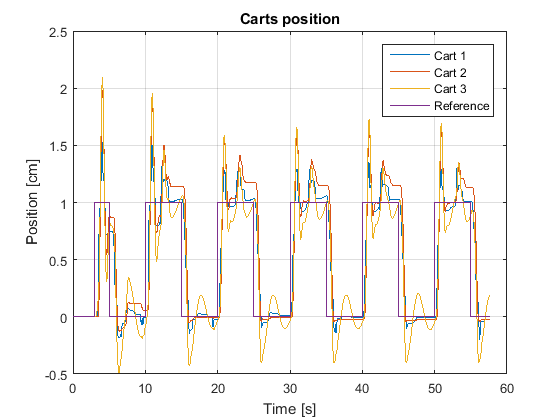
\includegraphics[width=0.5\linewidth]{img/hinf1.png}
\caption{Openloop frequency response from the motor input to the position of the second cart in the case of low and medium springs employed. The absence of the current loop yields an unacceptable response.}
\label{fig:hinf13dof}
\end{figure}

The regulator consists in a simple integrator $R(s)=\frac{50}{s}$, which is enough to stabilize the output current and achieve acceptable performance as shown in figure \ref{fig:hinf23dof}.


\begin{figure}[h]
\centering
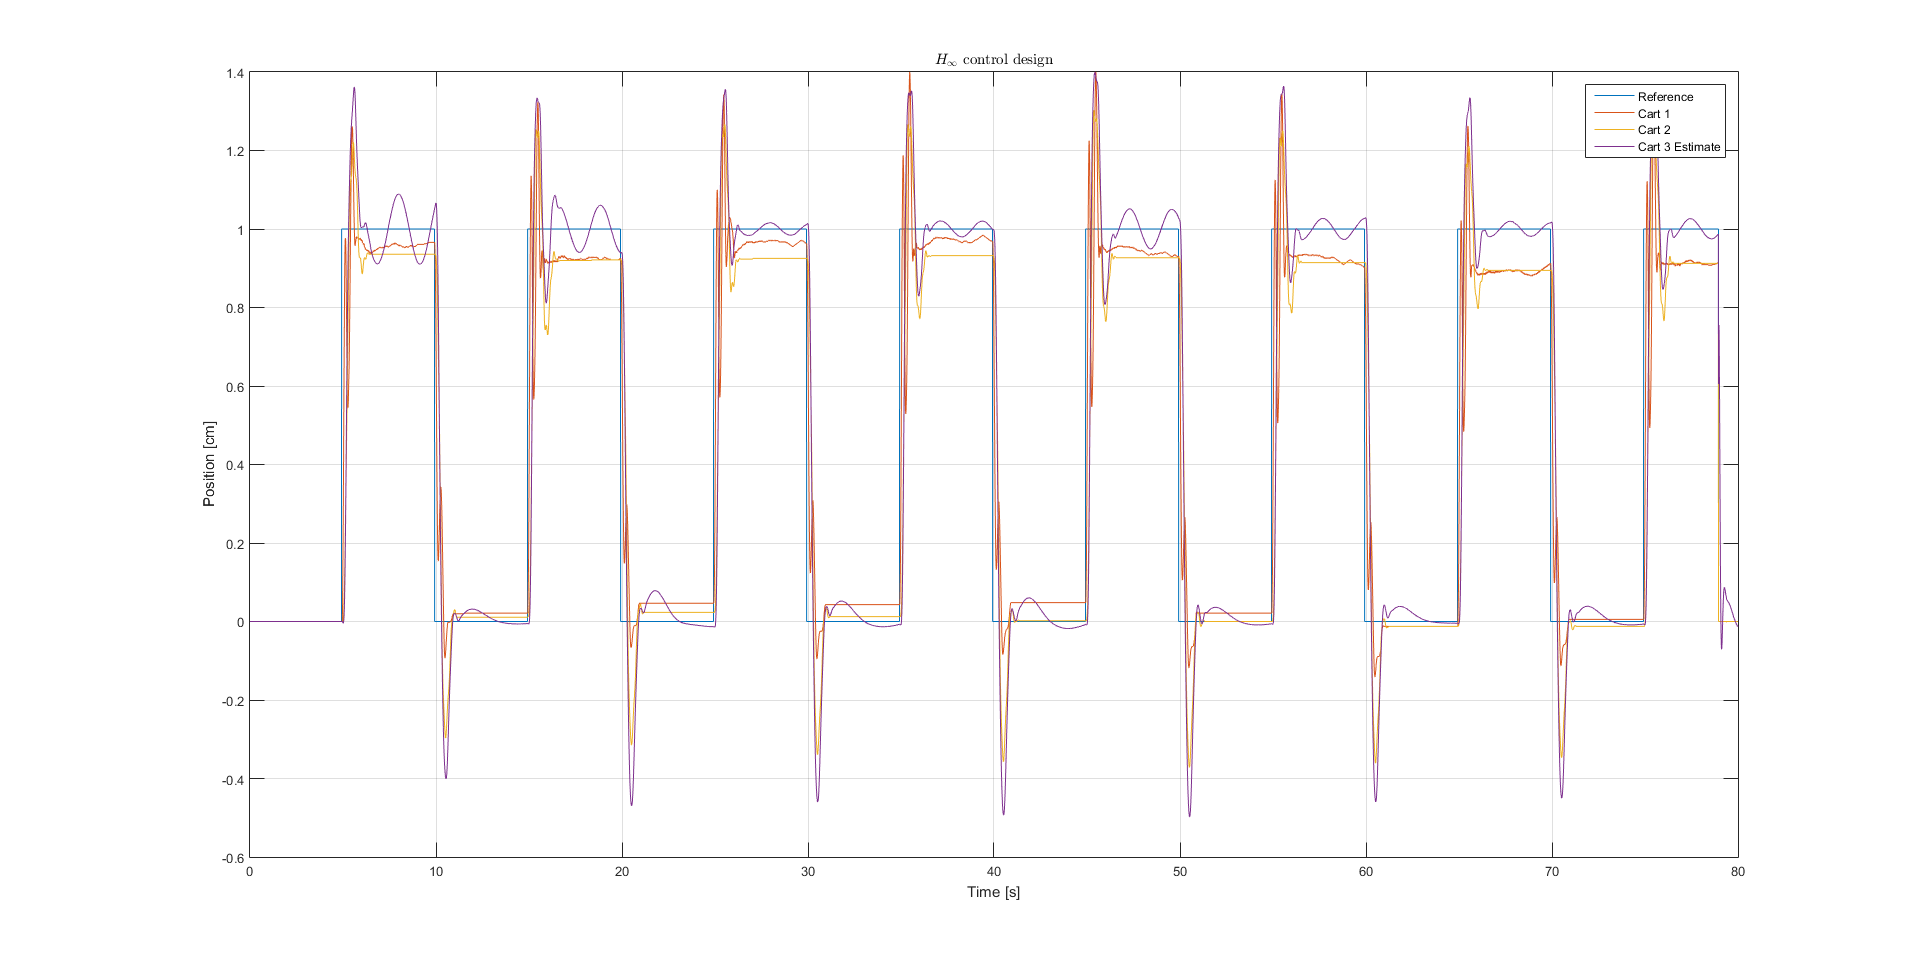
\includegraphics[width=0.5\linewidth]{img/hinf2.png}
\caption{Openloop frequency response from the motor input to the position of the second cart in the case of low and medium springs employed. The current loop gives a significant boost in performance.}
\label{fig:hinf23dof}
\end{figure}